\documentclass[journal]{vgtc}                % final (journal style)
%\documentclass[review,journal]{vgtc}         % review (journal style)
%\documentclass[widereview]{vgtc}             % wide-spaced review
%\documentclass[preprint,journal]{vgtc}       % preprint (journal style)
%\documentclass[electronic,journal]{vgtc}     % electronic version, journal

%% Uncomment one of the lines above depending on where your paper is
%% in the conference process. ``review'' and ``widereview'' are for review
%% submission, ``preprint'' is for pre-publication, and the final version
%% doesn't use a specific qualifier. Further, ``electronic'' includes
%% hyperreferences for more convenient online viewing.

%% Please use one of the ``review'' options in combination with the
%% assigned online id (see below) ONLY if your paper uses a double blind
%% review process. Some conferences, like IEEE Vis and InfoVis, have NOT
%% in the past.

%% Please note that the use of figures other than the optional teaser is not permitted on the first page
%% of the journal version.  Figures should begin on the second page and be
%% in CMYK or Grey scale format, otherwise, colour shifting may occur
%% during the printing process.  Papers submitted with figures other than the optional teaser on the
%% first page will be refused.

%% These three lines bring in essential packages: ``mathptmx'' for Type 1
%% typefaces, ``graphicx'' for inclusion of EPS figures. and ``times''
%% for proper handling of the times font family.

\usepackage{mathptmx}
\usepackage{graphicx}
\usepackage{times}

%% We encourage the use of mathptmx for consistent usage of times font
%% throughout the proceedings. However, if you encounter conflicts
%% with other math-related packages, you may want to disable it.

%% This turns references into clickable hyperlinks.
\usepackage[bookmarks,backref=true,linkcolor=black]{hyperref} %,colorlinks
\hypersetup{
  pdfauthor = {},
  pdftitle = {},
  pdfsubject = {},
  pdfkeywords = {},
  colorlinks=true,
  linkcolor= black,
  citecolor= black,
  pageanchor=true,
  urlcolor = black,
  plainpages = false,
  linktocpage
}

%% If you are submitting a paper to a conference for review with a double
%% blind reviewing process, please replace the value ``0'' below with your
%% OnlineID. Otherwise, you may safely leave it at ``0''.
\onlineid{0}

%% declare the category of your paper, only shown in review mode
\vgtccategory{Research}

%% allow for this line if you want the electronic option to work properly
\vgtcinsertpkg

%% In preprint mode you may define your own headline.
%\preprinttext{To appear in an IEEE VGTC sponsored conference.}

%% Paper title.

\title{Uncertainty and Trust Visualisation: TimeSets}

%% This is how authors are specified in the journal style

%% indicate IEEE Member or Student Member in form indicated below
\author{Saminu Salisu, Kai Xu, \textit{Adrian Wagstaff, Mike Biggs and Graham Phillips}}
\authorfooter{
%% insert punctuation at end of each item
\item
 Saminu Salisu is with Middlesex University . E-mail: s.salisu@live.co.uk.
\item
 Kai Xu is with Middlesex University, Inc.. E-mail: K.Xu@mdx.ac.uk.
\item
 Adrian Wagstaff and Graham Phillips are with Mass E-mail: AWagstaff@mass.co.uk.
}

%other entries to be set up for journal
\shortauthortitle{Biv \MakeLowercase{\textit{et al.}}: Global Illumination for Fun and Profit}
%\shortauthortitle{Firstauthor \MakeLowercase{\textit{et al.}}: Paper Title}

%% Abstract section.
\abstract{Timesets is a time series data visualisation application developed by \cite{timesets}, Timesets shows sequence of events displayed across a Timeline, while also makings sense of sets relations among events in the timeline \cite{timesets}. Timesets is very effective in identifying trends and sets relations within large set of time series events data. 
The current study looked into extending Timesets to accommodate visualisation of Trust and Uncertainty as part of its visualisation variables for events displayed across the timeline. The study is part of the UK Defence Solution Centre (UKDSC) sponsored autonomy and bigdata challenge in conjunction with the ministry of defence (MOD) through Defence Growth Partnership (DGP) Innovation Challenge with small and medium enterprises. The research study was carried out by Middlesex University and Mass. The aim of the proposed challenge is to develop a data analytic tool in the context of big data that can be used to aid military operations through intelligence analytics, data visualisation and decision making.
} % end of abstract

%% Keywords that describe your work. Will show as 'Index Terms' in journal
%% please capitalize first letter and insert punctuation after last keyword
\keywords{ Uncertainty, Trust, set visualization, timeline}

%% ACM Computing Classification System (CCS). 
%% See <http://www.acm.org/class/1998/> for details.
%% The ``\CCScat'' command takes four arguments.

\CCScatlist{ % not used in journal version
 \CCScat{K.6.1}{Computer Graphics & Visual Computing}%
{Data Visualisation}{Data};
 \CCScat{K.7.m}{The Computing Profession}{Miscellaneous}{Ethics}
}

%% Uncomment below to include a teaser figure.
  \teaser{
 \centering
 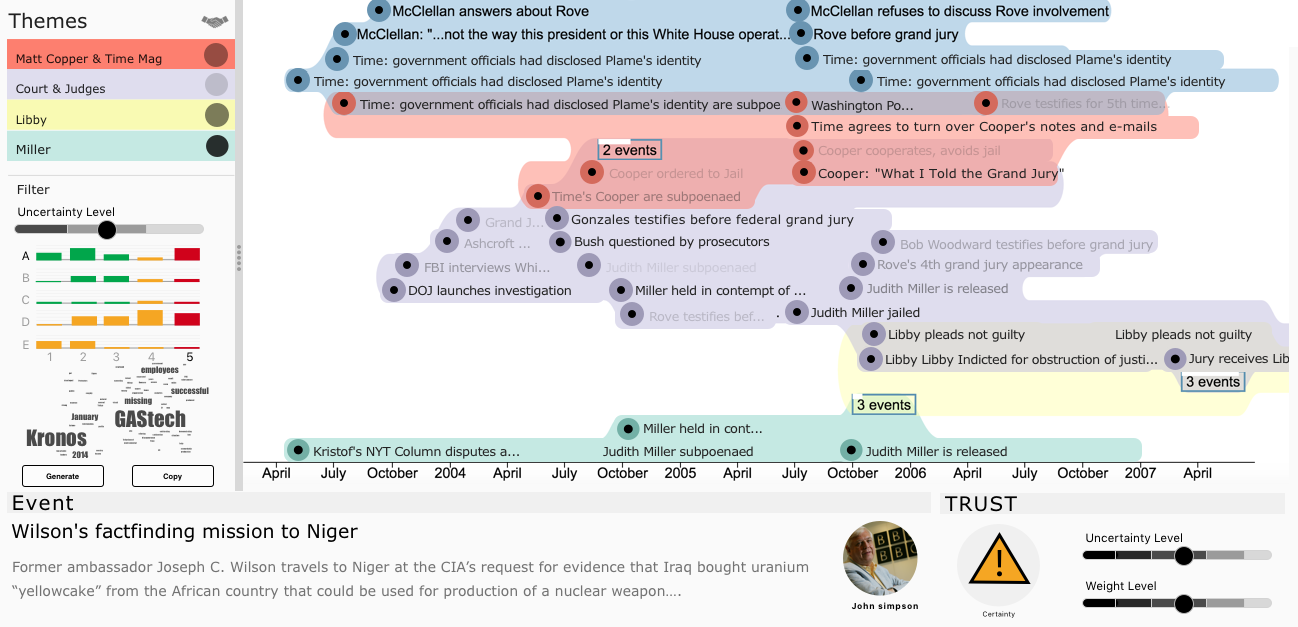
\includegraphics[width=16cm]{bg}
  \caption{: TimeSets visualization of the vast challange data showing Uncertainty and Trust in Data.}
  }

%% Uncomment below to disable the manuscript note
%\renewcommand{\manuscriptnotetxt}{}

%% Copyright space is enabled by default as required by guidelines.
%% It is disabled by the 'review' option or via the following command:
% \nocopyrightspace

%%%%%%%%%%%%%%%%%%%%%%%%%%%%%%%%%%%%%%%%%%%%%%%%%%%%%%%%%%%%%%%%
%%%%%%%%%%%%%%%%%%%%%% START OF THE PAPER %%%%%%%%%%%%%%%%%%%%%%
%%%%%%%%%%%%%%%%%%%%%%%%%%%%%%%%%%%%%%%%%%%%%%%%%%%%%%%%%%%%%%%%%

\begin{document}
\firstsection{Introduction}

\maketitle
TimeSets consist of a timeline showing sequence of events displayed across a visualisation, while makings sense of sets relation among events in the timeline \cite{timesets}. Time set is very effective in identifying trends and sets relations within a large set of events. 

The Study looked into extending Time Set to accommodate Visualisation of Trust and Uncertainty as parts of its variables for events displayed across the Timeline. The above study is part of the UKDSC Autonomy and Big data sponsored by the ministry of defence through Defence Growth Partnership (DGP) Innovation Challenge with small and medium enterprises carried out by Middlesex University and Mass. The aim of the challenge is to build tools in the context of big data analytics that can be used to aid military operations through intelligence analytics and decision-making. 

The paper begins with a review of related literature in the area of Uncertainty, Trust and Time series Visualisation with focus in the area of Uncertainty Visualisation and Variables that can be used to identify uncertainty in a visualisation, followed by trust perception models in general principle, user observation to test out the research hypothesis and workshops where carried out to develop uncertainty and trust design variables with the security and defence sector as the target users.

\section{Related Work}

\subsection{Trust Perception}

Uncertainty and Trust has been the subject of less extensive research compared to data mining and extraction, while it is beyond the scope of this paper to provide a complete overview of research in Uncertainty and Trust, in the following section, we describe aspects of the research on Uncertainty and Trust propagation, we also review more recent literature on the role of Uncertainty and Trust and in Trust models and Finally, we briefly review finding from the research study carried out.

Some of the first attempts to quantify user perception of trust were carried out in a study by \cite{trust-perception}, although previous studies where geared towards identifying the sets of factors influencing trust, the author took the novel approach of quantifying the value of each trust factor in a given domain. The result of the study can enable visualisation interface developers to focus on key elements that influence trust and increase the trustworthiness of an interface. 

Trust is an important aspect of interaction between people and systems \cite{fuzzy-trust}, Various mechanisms have been used to Visualise trust in different domains such as the trust ratings employed by auction sites to other dealers. Although current mechanisms for trust inference commonly try to compute a global trust, the study by \cite{fuzzy-trust} suggest the precise modelling of trust between two entities.  

Similar study by \cite{recommender-study} in the area of recommender system looked into the effects of real time feedback based on a controlled study of profile manipulation and measure the effects on the resulting recommendation and general users experience. The results from the study suggests that real time feedbacks improves perceived accuracy of recommendation regardless of the quality of the actual recommendation \cite{recommender-study}. 

Also the study by \cite{trust-relationships} suggest the use of pop-ups visualisation of trust network on e bay market place. The author also suggest ascertain even the use of small lexicon important features on the market place about the product improved perception exponentially.  

\subsection{Visualising Uncertainty}
The Study carried out by \cite{uncertainty-graphedges} looks into visual variables used to represent uncertainty. 
The paper reports on a study carried out about the perception of graph edge attributes when uncertainty associated with each edge and the main edge attribute are visualized simultaneously using two separate visual variables, Some of the results show that factors such as Grains, fuzziness and Transparency depict uncertainty effectively.

Visual Representation of uncertainty with focus on variables that can be used to depict uncertainty and trust in data is key to support the design study. An experiment carried out by \cite{visualising-uncertainty} to determine the effectiveness of uncertainty variables such Grains, fuzziness and Transparency led to some generalised conclusion by the author, Fuzziness and Variable locations work very well in uncertainty visualisation, Values and arrangement of variables are also an effective means of showing uncertainty. Transparency and variable sizes are theoretically valuable for representing uncertainty.

Visualising uncertainty in other domains is also a key consideration for the design due to the wide range of digital devices used to access software?s and applications both in and outside the military industries. The study by \cite{bus-uncertainty} proposed a novel design quantile dotplots interface in the mobile context for presenting uncertainty in real-time transportation with main focus on transit arrival times.  quantile and dotplots was shown to improve estimation of transit time arrival by end-users in a controlled experiment \cite{bus-uncertainty}. 

Another study by \cite{uncertainty-aware-multidimensional-data} looks into modelling and exploration in multidimensional data. The author presents an efficient visualization and exploration approach for modelling and characterizing the relationships and uncertainties in the context of a multidimensional ensemble dataset. The author focuses more on simulation and analysis with some suggestion on using ensemble simulation to study uncertainty.

Theme Delta \cite{themedelta} is another timeline visualisation data similar to time sets but uses sinuous, variable-width lines to show this evolution on a timeline, utilizing colour for categories, and line width for keyword strength.
The study focuses on the Visualization of data over time with focus on temporary data that has a life spam and can have reduced value over time. In relation to the user observation study carried out, data life span affect the uncertainty level of that data over time.

\section{Methodology}

\subsection{Study Design}
\subsubsection{User Observation}

To determine users perception of Uncertainty and Trust in Data, Pair analytics research method for observational exploratory exercise was used to observe the interaction between a subject and a controller  \cite{pair-analytics} . Pair analytics is a research method used for visual analytic reasoning and collaboration. Pair analytic is carried out by two participants, the Subject Matter Expert (SME) and Visual Analytics Expert (VAE), the VAE plays the role of the observation controller/driver while the SME controls the VAE as the navigator in an exploratory data analysis task which involved analyses of data from VAST Challenge 2014 Mini Challenge 1.

VAE was exposed to a visual interface for visualisation while using the legacy version of the TimeSets for timeline data analysis, Kebana for quick search and SenseMap for hypothesis building. The subjects where also instructed to ask question directly to the VAE that they deemed relevant to the performance of their data analysis task. The subjects were allowed to communicate and encouraged to think-aloud without any restrictions as they used the tools to analyse the data from the challange and to  answer the follow up question.

VAE Users where given a complete description of the challenge data, problem description, access to computers with TimeSets, Kebana and SenseMap on double desktop display screen as seen in the figure below. The environment setup ensured VAE and the SME had access to multiple visualisation and the necessary tools to address the questions set out in the VAST challenge 2014 Mini Challenge 1.

\begin{figure}[htb]
 \centering
 \includegraphics[width=3.5in]{img/obs1}
 \caption{A subject examining a legacy version of Timesets with the DAC (Data Analyst controller) depicting the Vast 2014 mini challange data in an observational, exploratory user study to enable visual data exploration}
\end{figure}

\begin{figure}[htb]
 \centering
 \includegraphics[width=3.5in]{img/obs2}
 \caption{DAC (Data Analyst controller) asks the subject question and feedback on how they handled uncertainty presented by the Vast challenge data as part of the user observational study }
\end{figure}

\subsubsection{Workshops}
The design workshops where aided with the use of Sprint Design to simply brainstorm design ideas in cooperation with agile environment.

\begin{figure}[htb]
 \centering
 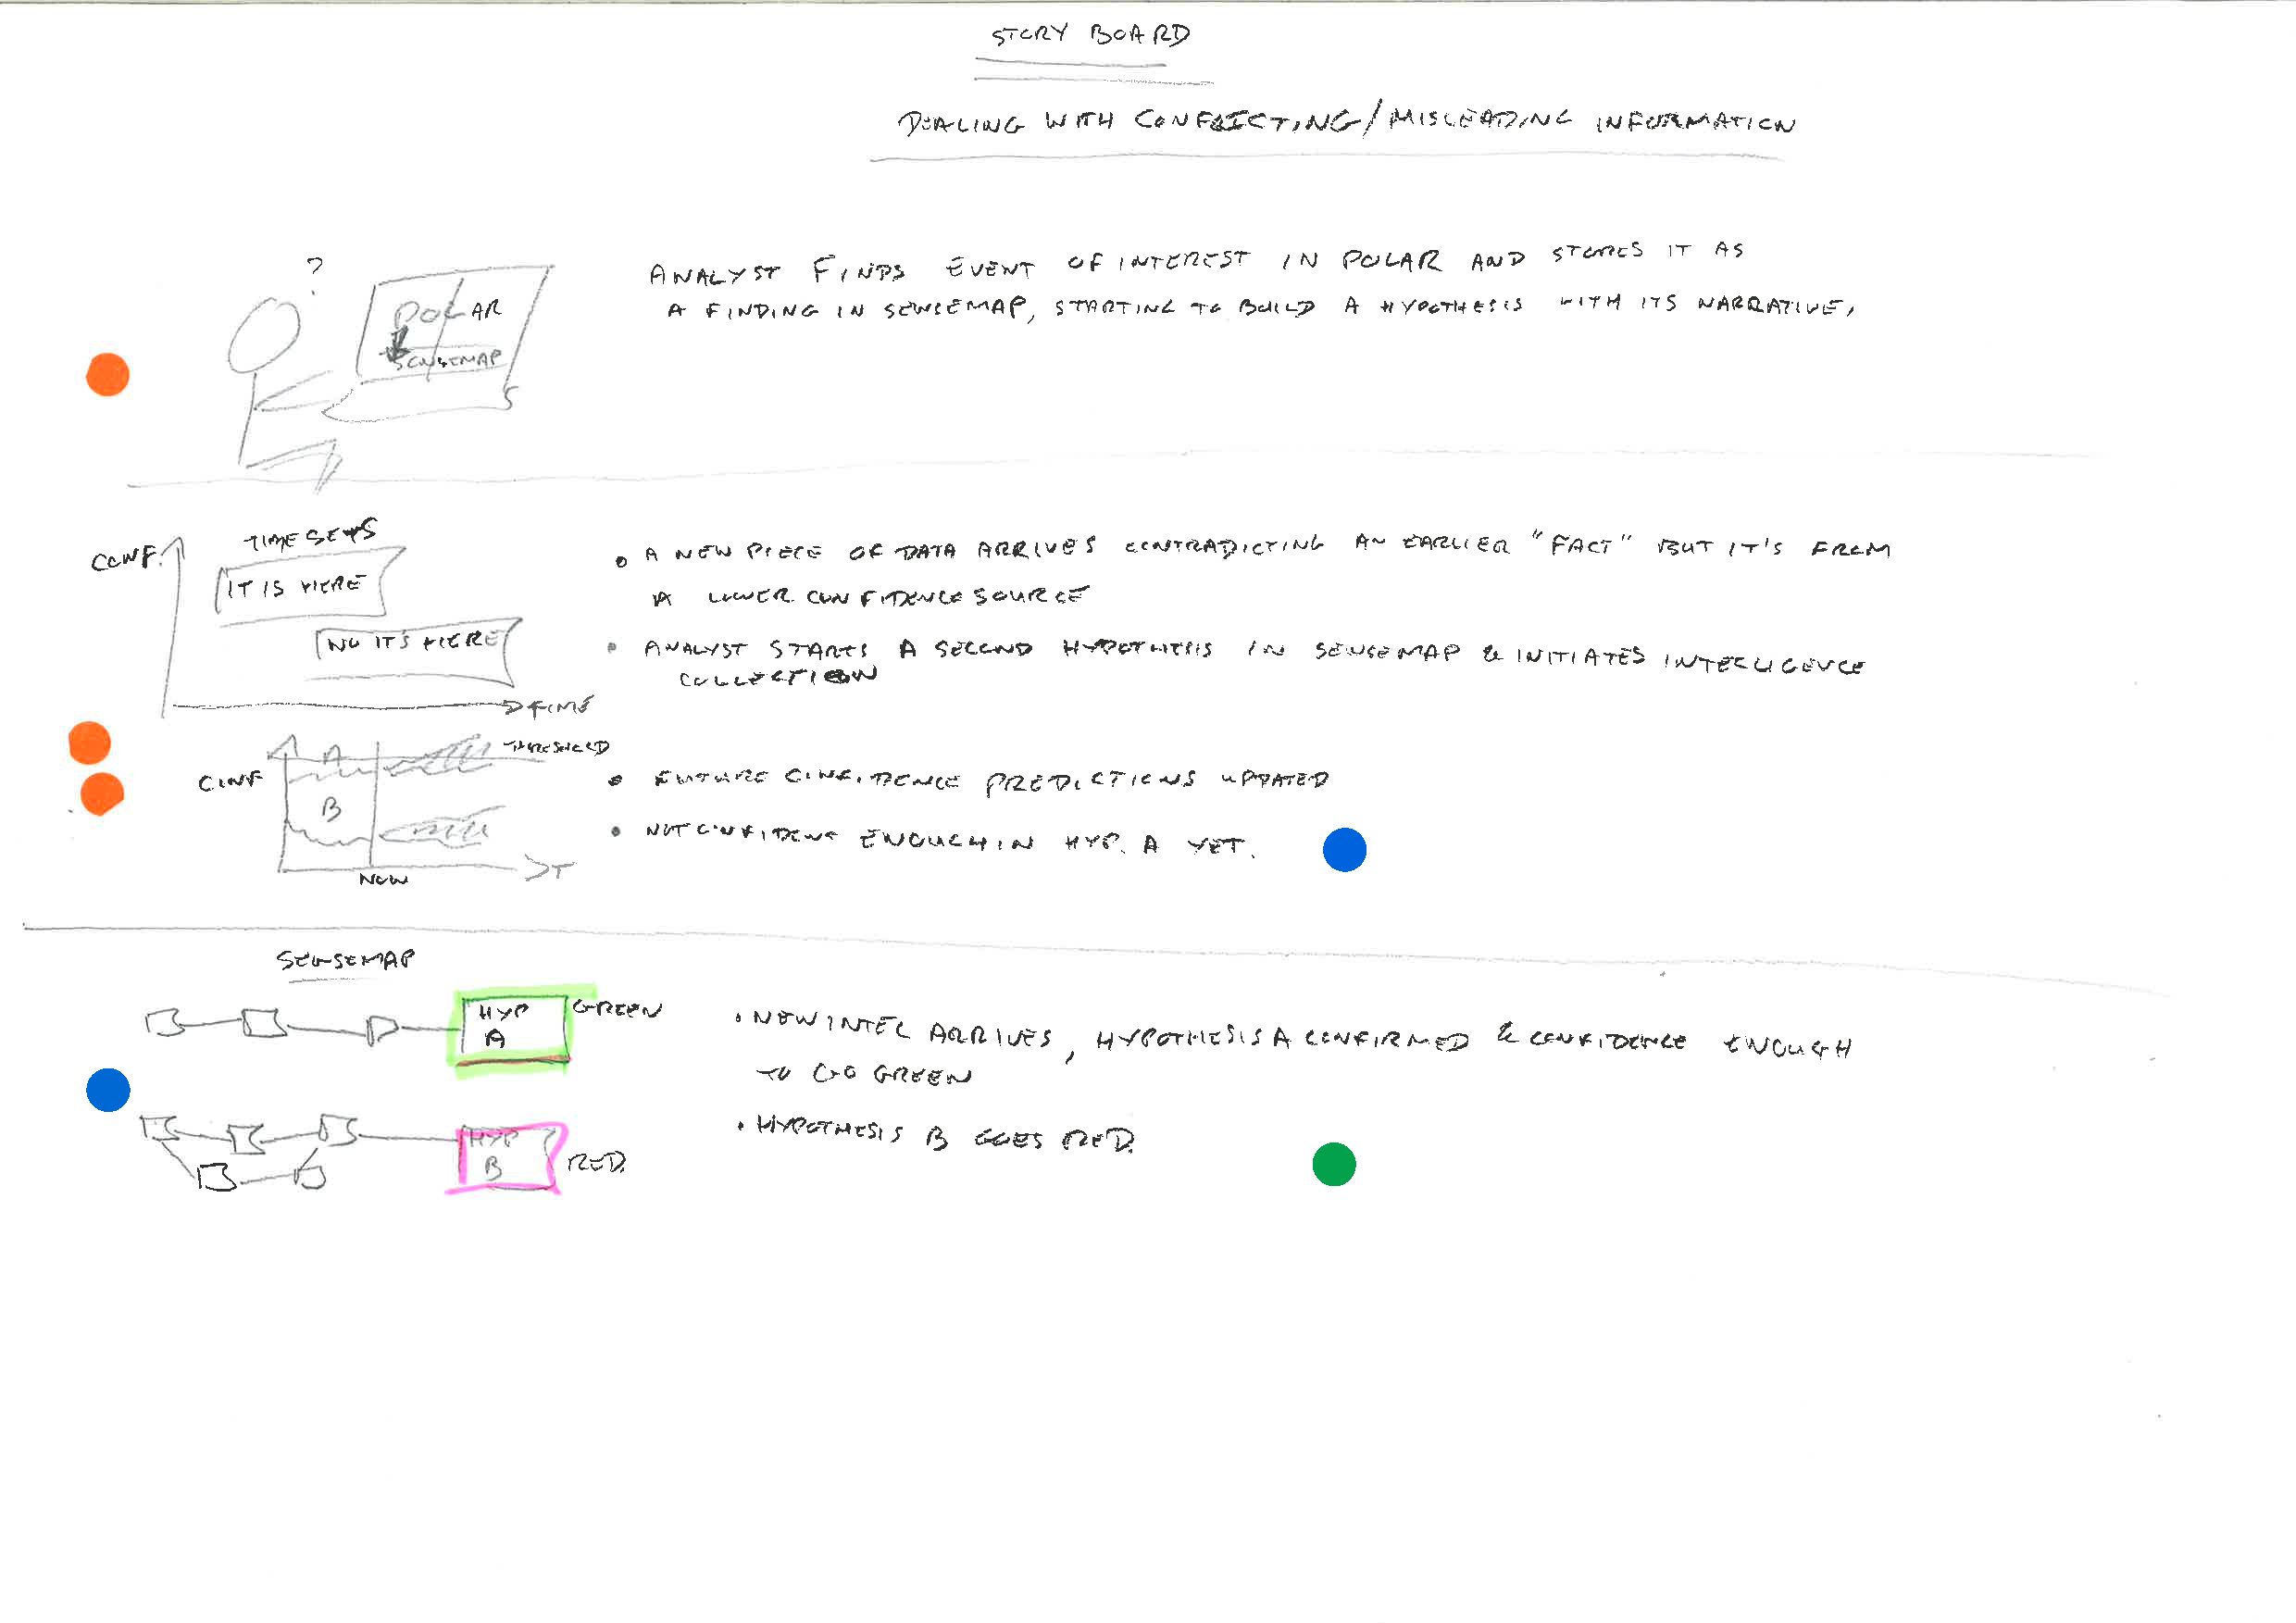
\includegraphics[width=3.5in]{img/adrian}
 \caption{ Story Board 1: }
\end{figure}

\begin{figure}[htb]
 \centering
 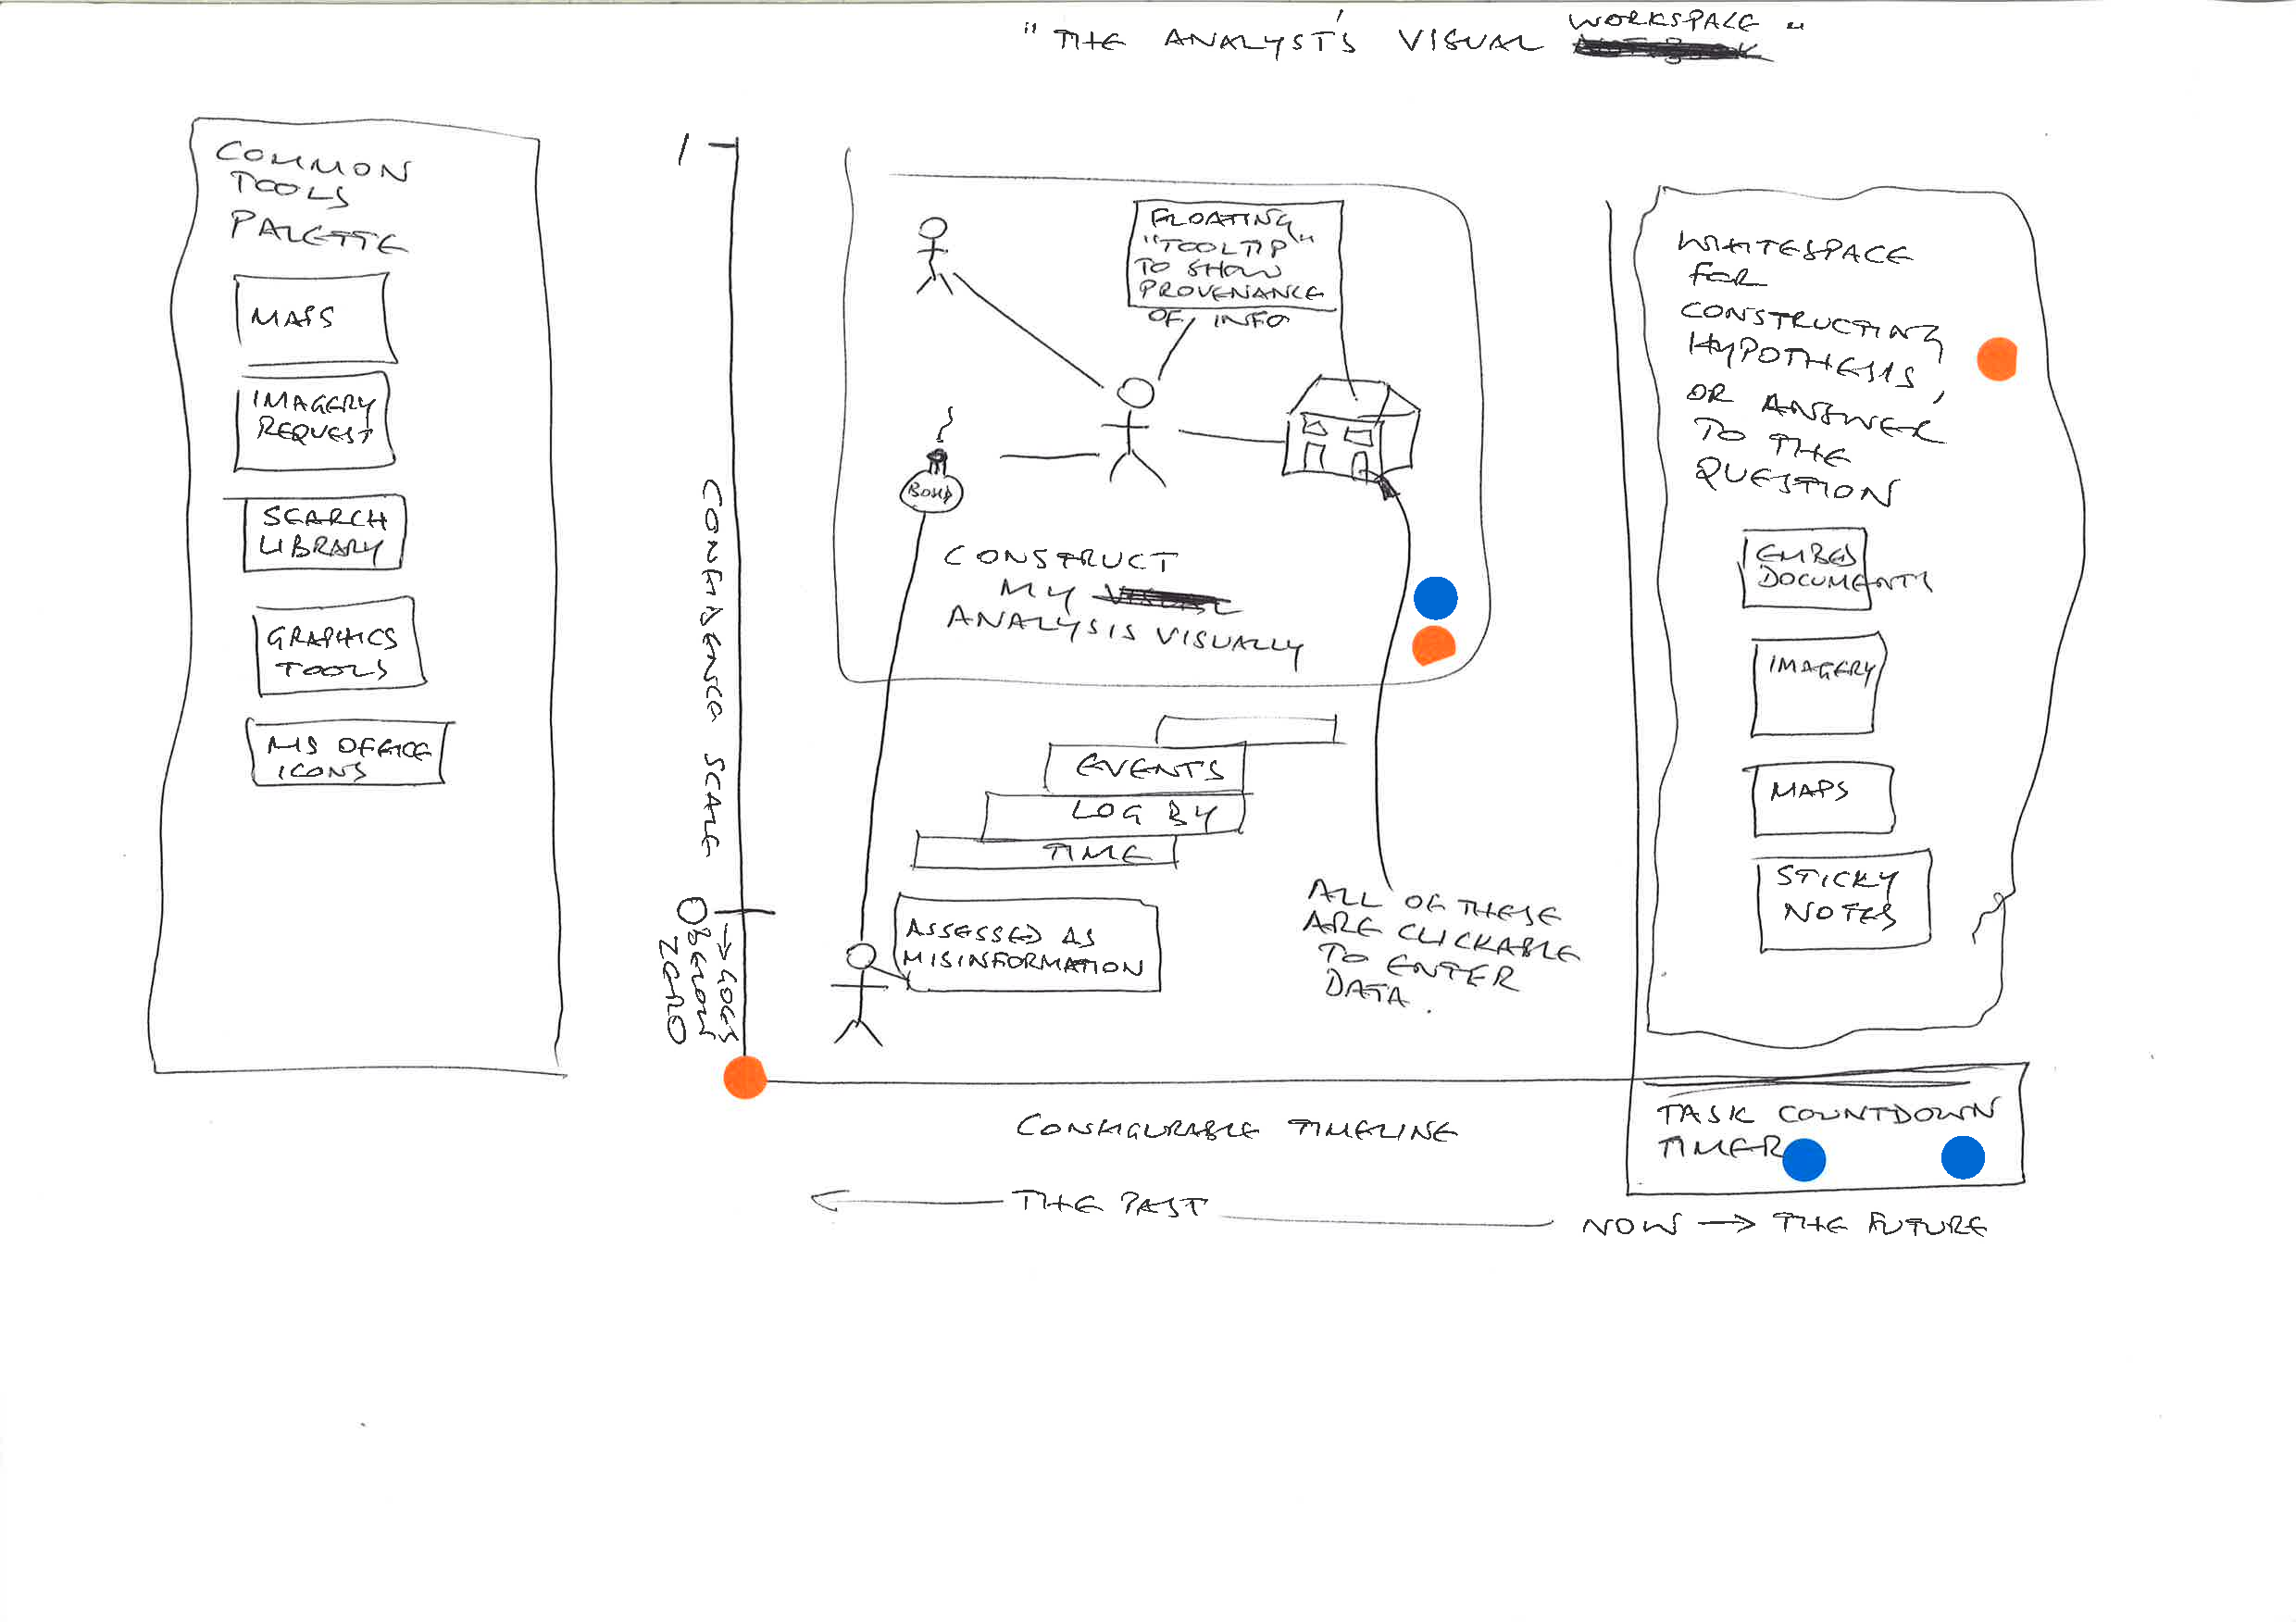
\includegraphics[width=3.5in]{img/james}
 \caption{ Story Board 2: }
\end{figure}

\begin{figure}[htb]
 \centering
 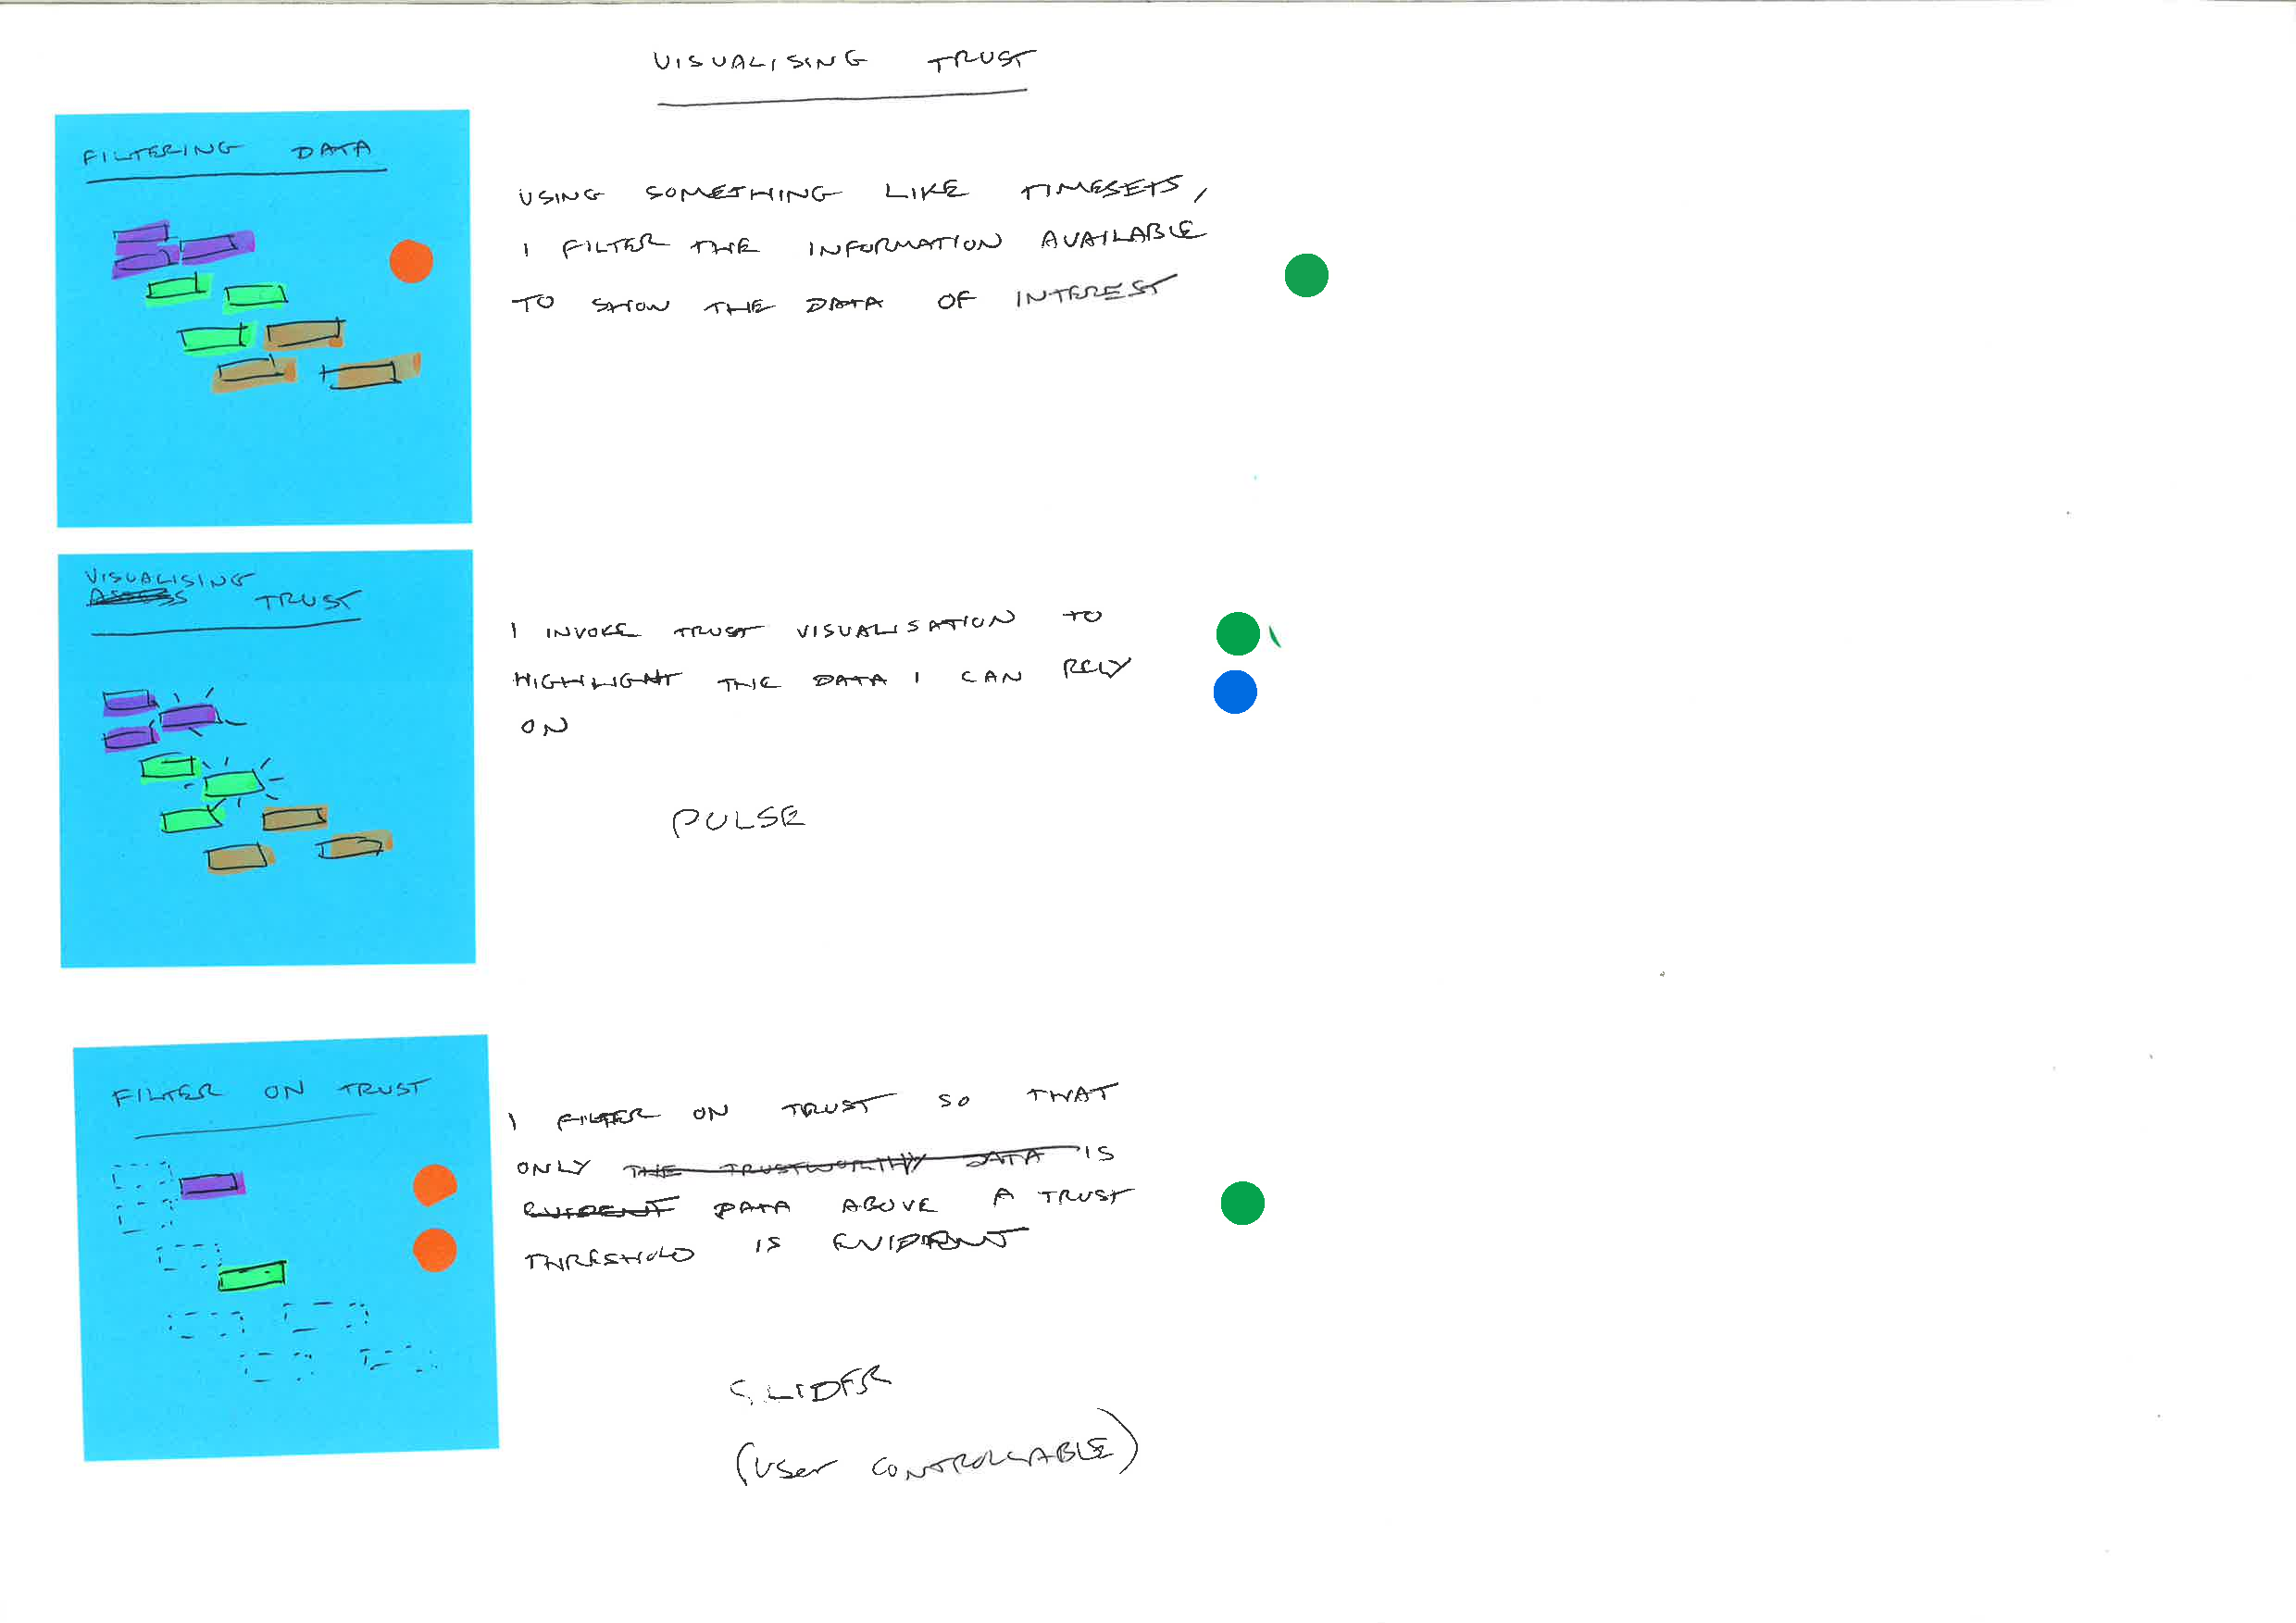
\includegraphics[width=3.5in]{img/mike}
 \caption{ Story Board 3: }
\end{figure}


\subsection{Participants}
3 pilot studies where conducted which included 1 user observation and 2 workshops to refine the experimental design. The participating subjects in the User Observation are 2 Experienced data analyst with vast experiences in the military sector, both male aged between 40 and 55 which lasted for about 3 hours each. Participants had varied experience with the challenge and data analysis with one participant an ex-army analyst and ex-raf analyst respectively.

The participants for the workshops consist of 1 ex-army chief, 3 researchers, 1 project manager and 1 developer with each participant showing moderate familiarity with uncertainty and information visualisation.

\subsection{Data Analysis Approach}
\subsubsection{Approach}
Due to the limited number of participants, inferential statistical approach was adopted for this research. Inferential statistics analyses data that researches have limited access to, as a result they use procedures to infer the meaning on collected data from a given population, it is used when it is essential to analyse behavioural statistics of a given population

\subsubsection{Models: Coding}
Coding method involves the transcription of data collected from the user observation and interviews through audio / video recording to short written scripts that can be used to make analysis. Data collected using qualitative method such as the interviews with the Participants during the User Observations are analysed in coding by segmenting the response into meaningful variables and assigning those variables into categories know as a code.\\

The following codes where created to enable easy analysis of the data collected from the interview with the participants. The analysed result can be found in the next section of this report

\begin{enumerate}
  \item Types or Variations of uncertainty
  \item Marking or Recording uncertainty
  \item Benefits of uncertainty to Reasoning and thinking
  \item Challenges in dealing with uncertainty
\end{enumerate}

\subsubsection{Tools: Thematic}
Using thematic to monitor, examine and record theme patterns across the collected data from the qualitative research analysis.
Thematic is best used to emphasise on the subject?s use and awareness of the key elements that derives uncertainty and trust in data presented to the analyst.
Contribution by the researchers in the data analysis stage using thematic method that requires looking out for patterns/themes in the data. Few factors has to be put into consideration: What is the size of the theme, what counts as a pattern/theme, Identifying the key themes, what are the key questions of interest in relation to uncertainty visualization.

To determine the answer to the above questions, the following themes and patterns where identified from the analysis of the result in interviews carried out with the participants during the user observation.

\begin{enumerate}
  \item Source of Data is key to trust and certainty
  \item Experienced MOD users are comfortable with dealing with uncertainty
  \item New source of information increases confidence level over time
  \item Internal and known source of information more trusted than external source data
  \item Aligning high confidence hypothesis on the top of low confidence hypothesis
  \item Icon or component for marking confidence level in hypothesis
  \item Familiarity impact the approach and use of tools
\end{enumerate}

\subsection{Initial Findings}
\subsubsection{Data source as a key factor to confidence}
The observation study of the two participants enabled the researchers to identify data source as a key element that affect uncertainty and trust as agreed by both participants. 
\begin{enumerate}
  \item Both participants agree that the source of data is key to confidence in that data
  \item Different data sources have different levels of trust 
\end{enumerate}

\subsubsection{Updated source of information affects confidence level overtime}
As the study progressed, continuous discovery of new and updated information changed the participant?s confidence in that data. Both participants regardless of their approach to the solving the data challenge constantly referred back to time sets and Kebana for new information sources that will further support or refute the derived hypothesis.

\subsubsection{Internal and known sources are more trusted than external sources}
The response of increased confidence in a data from participant (J) when he discovered a source of information with the label (psycops) indicates that a form of label or logo showing who reviewed an information can significantly increase the level uncertainty and trust in that data. Some of the key points to further prove these points are below
\begin{enumerate}
  \item Both participants agree news report form specific companies where more trusted than others just by identifying with the companies logo or brand
\end{enumerate}

\subsubsection{Uncertainty and Trust variables}
Both participants at some point during the study wanted to identify the level of uncertainty by marking the confidence in hypothesis so as to remember, which further indicates the importance of showing confidence levels using variables such as transparency, hue, saturation, on hypothesis and data used to derive the hypothesis. 

\subsubsection{High Confidence before Low Confidence Arrangement }
The user observation also highlighted the importance uncertainty arrangement by confidence level with high-level confidence information placed above on-top and low level information placed on the bottom. One of the participants consistently reflected this by placing all high-level hypothesis above less confident hypothesis in Sense Map. 

\subsection{Reflection}
The user observation has enabled the researchers to gain valuable insight into users perception of uncertainty different ways in which uncertainty is being handled during decision-making in relation to data analysis. The observation also identified and recommends some effective methods and techniques of communicating uncertainty in data during analysis by identifying key elements that constitute uncertainty and ways they can be communicated across the decision making circle in the military data intelligence and information consumption. 

\section{Latest Timesets Updates}

The new Version of Timesets design was guided by the work carried in the study. the design shows new component indicating uncertainty and trust in data. some of this component include 


\begin{enumerate}
  \item Transparency to indicate uncertainty in events by using opacity to gauge level of trust in data. high opacity indicates high confidence while low opacity shows low confidence in data
  	\begin{figure}[htb]
 	\centering
 	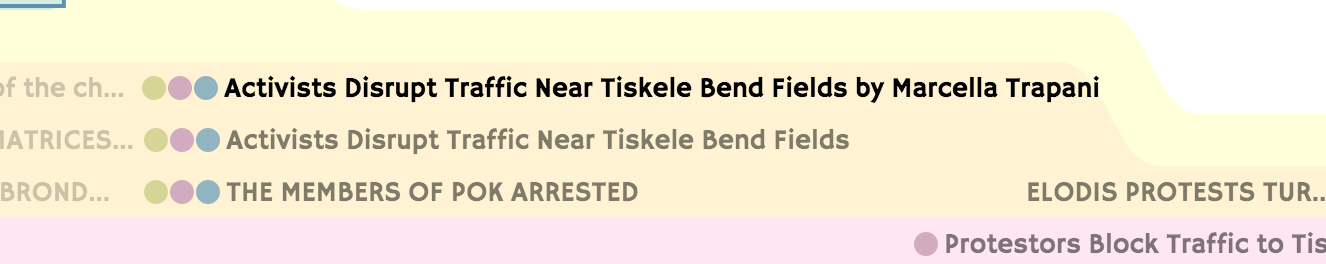
\includegraphics[width=3.5in]{img/transparency}
 	\caption{ Figure showing high Opacity and low opacity events indicating uncertainty levels}
	\end{figure}

  \item Trust Histogram to indicate the 5x5x5 trust model in the shape of an histogram. This histogram can be used to indicate source evaluation with A showing indicating "always reliable"  and E indicating "Untested Source"
  \begin{figure}[h!]
 	\centering
 	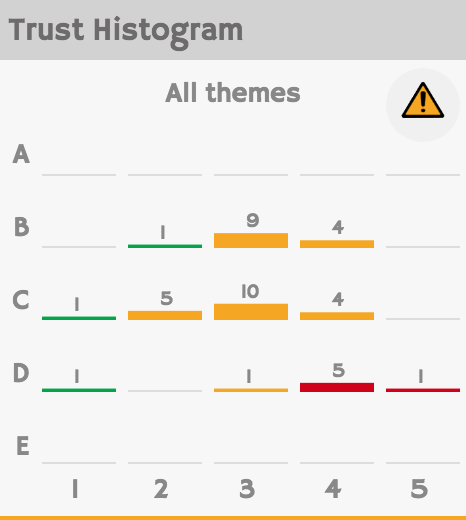
\includegraphics[width=1.0in]{img/histogram}
 	\caption{ Figure showing Trust Indicators on Themes}
	\end{figure}
  
  \item Trust Indicators on set Themes to show the average level of trust in a group of events. This is indicated by the the triangle and colour of the triangle with Green standing for high level of trust and Red for Low level of trust  
  	\begin{figure}[htb]
 	\centering
 	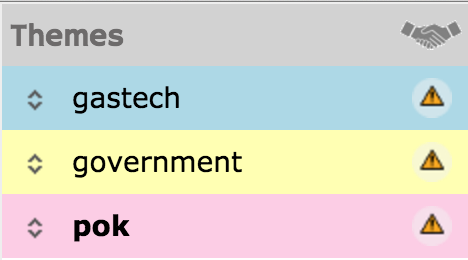
\includegraphics[width=1.0in]{img/themes}
 	\caption{ Figure showing Trust Indicators on Themes}
	\end{figure}
	
  \item Trust Filter used to filter only events with specific levels of trust based on three categories, Low, Medium and High.
    	\begin{figure}[htb]
 	\centering
 	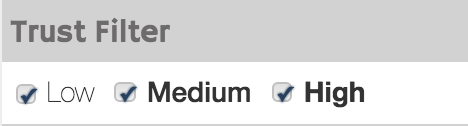
\includegraphics[width=1.0in]{img/filter}
 	\caption{ Figure showing Trust Filters for Low, Medium and High events}
	\end{figure}
  
  \item Icon/Logo display as part of article viewer which increases trust in data as supported by the result from the user observation from the Initial Findings 
  \item User modified slider that can be used to adjust the level of Trust and Uncertainty attached to an and event or data
\end{enumerate}

\section{Evaluation}


\section{Conclusion}
The user observation has enabled the researchers to gain valuable insight into users perception of uncertainty different ways in which uncertainty is being handled during decisionmaking in relation to data analysis. The observation also identified and recommends some effective methods and techniques of communicating uncertainty in data during analysis by identifying key elements that constitute uncertainty and ways they can be communicated across the decision making circle in the military data intelligence and information consumption. 

%% if specified like this the section will be committed in review mode
\acknowledgments{
The authors wish to thank A, B, C. This work was supported in part by
a grant from the UKDSC and mass.}

\vspace{6cm}

\bibliographystyle{abbrv}
%%use following if all content of bibtex file should be shown
%\nocite{*}
\bibliography{ref/CGVC}

\end{document}
